\documentclass[11pt]{article}

\usepackage{fontspec}
\setmainfont{Apple SD Gothic Neo}
\setmonofont{Menlo}[Scale=0.85]
\newfontfamily\latinfont{Times New Roman}
\newcommand{\Jorda}{{\latinfont Jordà}}

\usepackage[a4paper,margin=2.3cm]{geometry}
\usepackage{graphicx}
\usepackage{booktabs}
\usepackage{array}
\usepackage{float}
\usepackage{caption}
\usepackage{amsmath}
\usepackage{xcolor}
\usepackage[hidelinks]{hyperref}
\usepackage{enumitem}

\definecolor{accent}{HTML}{2c6fbb}
\captionsetup{font=small,labelfont={bf,color=accent}}
\setlist{nosep,leftmargin=1.4em}
\graphicspath{{fig/}}
\linespread{1.12}

\title{\vspace{-1.2cm}\textbf{시장 지수 시그널 탐색 실험 보고서}\\[4pt]
\large TimesFM 예측력 \textperiodcentered\ 푸리에 주기성 \textperiodcentered\ 거시 이벤트 충격반응}
\author{Croesus Research --- 탐색 실험(throwaway exploratory)}
\date{2026년 6월 30일}

\begin{document}
\maketitle
\vspace{-0.6cm}

\begin{abstract}
\noindent
본 보고서는 미국 주가지수(S\&P~500, NASDAQ)에 대해 세 가지 독립적인 탐색 실험을 수행한 결과를 정리한다.
\textbf{(1)} 구글의 시계열 파운데이션 모델 \emph{TimesFM}이 지수 예측에 쓸 만한지,
\textbf{(2)} 지수에 통계적으로 유의한 \emph{반복 주기}가 존재하는지(푸리에 분석),
\textbf{(3)} 전쟁\textperiodcentered 팬데믹\textperiodcentered 관세\textperiodcentered 원유 같은 거시 충격이 지수에 미치는 \emph{영향의 크기(magnitude)와 지속 기간(period)}을 정량화할 수 있는지를 검증하였다.
핵심 결론은 다음과 같다. TimesFM은 \emph{방향성}에서는 단순 추세(drift) 기준선을 모든 구간에서 5--10\%p 앞서지만, \emph{점 예측의 오차(RMSE)}는 random walk보다도 크다(변동폭 과대추정). 즉 방향 신호로서는 가능성이 있으나 가격 예측기로는 부적합하다. 푸리에 분석에서는 전처리 후 ``유의''하게 검출된 피크 수가 우연 기대치와 사실상 같아, \emph{신뢰할 만한 반복 주기는 발견되지 않았다}(스펙트럼상 red noise와 구분 불가). 이벤트 분석에서는 사건 연구(CAAR)와 \Jorda{} 국소투영(local projection)으로 충격반응함수를 추정하여, 팬데믹($\approx-40\%$, 느린 회복)과 원유(지속적 약세)는 뚜렷한 음(-)의 충격을, 전쟁\textperiodcentered 관세는 얕은 초기 하락 뒤 표본 내에서 오히려 양(+)의 표류를 보였다(소표본, 넓은 신뢰구간).
\end{abstract}

\section{서론}

Croesus 파이프라인에 ``참고할 만한 시그널''을 추가할 수 있는지 가늠하기 위해, 본 작업은 세 가지 질문을 각각 독립 실험으로 검증한다. 모든 실험은 일회성 탐색(throwaway)을 목적으로 하며, 메인 패키지에 통합하지 않고 \texttt{experiments/market\_signals/} 아래에서 결과(CSV/PNG)와 결론(\texttt{FINDINGS.md})만을 산출한다.

\begin{enumerate}[label=\textbf{Q\arabic*.}]
  \item \textbf{TimesFM} --- 파운데이션 시계열 모델이 지수 수익률 예측에서 순진한 기준선을 이기는가?
  \item \textbf{푸리에} --- 지수에 반복적으로 나타나는 주기가 실제로 존재하는가, 아니면 착시인가?
  \item \textbf{이벤트 임팩트} --- 거시 충격의 크기와 지속 기간을 측정할 수 있는가?
\end{enumerate}

\paragraph{방법론적 전제(중요).}
Q3의 최초 아이디어는 ``푸리에로 다른 이벤트를 걸러내고 특정 이벤트의 주파수만 분리''하는 것이었으나, 이는 신호처리 관점에서 적절치 않다. 전쟁\textperiodcentered 팬데믹\textperiodcentered 관세\textperiodcentered 원유 쇼크는 \emph{일회성 충격(impulse/step)}이지 \emph{주기 신호(periodic)}가 아니므로 분리할 ``주파수''가 존재하지 않는다. ``충격의 크기와 지속''을 묻는 올바른 도구는 \emph{사건 연구}와 \emph{국소투영 충격반응함수}이며, Q3는 이를 사용한다. 반면 ``반복 주기가 있는가''는 본질적으로 스펙트럼 질문이므로 Q2에서 푸리에를 사용한다.

\section{데이터 및 공통 방법}

\paragraph{데이터.} 가격은 yfinance에서 수집하여 DuckDB(\texttt{storage/croesus.duckdb}, \texttt{prices\_daily} 테이블)에 read-through 캐시한다. 대상은 S\&P~500(\texttt{\^{}GSPC})과 NASDAQ Composite(\texttt{\^{}IXIC})의 \emph{수정 종가 일봉}이다. 실험별 사용 구간은 푸리에 1971--2026, 이벤트 1985--2026, TimesFM 2005--2026이다.

\paragraph{공통 전처리(detrend).} 전처리를 1급 객체로 분리하여 \emph{전처리 유무를 나란히 비교}할 수 있게 하였다. 세 가지 변환을 제공한다:
\begin{itemize}
  \item \texttt{identity} --- 무처리 기준선(로그 가격 그대로).
  \item \texttt{demean\_logret} --- 로그 수익률에서 평균 성장률(drift)을 제거($\Delta\log P - \overline{\Delta\log P}$).
  \item \texttt{detrend\_linear} --- 로그 가격에서 선형 추세를 적합 후 제거한 잔차.
\end{itemize}

\section{실험 1 --- TimesFM 예측력 평가}

\subsection{방법}
가격 \emph{레벨} 예측은 가격의 관성 때문에 무조건 그럴듯해 보이는 함정이 있다. 따라서 \emph{수익률/방향}을 평가하고 순진한 기준선과 비교한다.
\begin{itemize}
  \item \textbf{프로토콜:} rolling-origin out-of-sample. 각 시점에서 컨텍스트(512 거래일)를 입력해 1\textperiodcentered 5\textperiodcentered 21 거래일 앞을 예측. 시점 간 간격 21일($n=232$ 표본).
  \item \textbf{기준선:} random walk(마지막 값 유지 $\rightarrow$ 수익률 0), drift(평균 로그성장률 연장).
  \item \textbf{지표:} 수익률 RMSE, 방향 적중률(hit rate), random walk 대비 skill score $=1-\text{RMSE}_\text{model}/\text{RMSE}_\text{RW}$.
\end{itemize}

\subsection{결과}
\begin{table}[H]\centering\small
\caption{TimesFM 대 기준선 --- 구간별 방향 적중률, RMSE, RW 대비 skill ($n=232$). 적중률은 높을수록, RMSE는 낮을수록 좋다.}
\begin{tabular}{llrrrrr}
\toprule
지수 & 구간 & TimesFM hit & drift hit & TimesFM RMSE & RW RMSE & skill vs RW \\
\midrule
S\&P 500 & 1d  & 55.2\% & 50.0\% & 0.0131 & 0.0118 & $-0.107$ \\
S\&P 500 & 5d  & 66.4\% & 56.5\% & 0.0276 & 0.0252 & $-0.093$ \\
S\&P 500 & 21d & \textbf{70.3\%} & 60.8\% & 0.0638 & 0.0486 & $-0.313$ \\
\midrule
NASDAQ  & 1d  & 51.3\% & 46.6\% & 0.0214 & 0.0126 & $-0.698$ \\
NASDAQ  & 5d  & 63.4\% & 54.3\% & 0.0583 & 0.0283 & $-1.065$ \\
NASDAQ  & 21d & \textbf{67.7\%} & 60.3\% & 0.0816 & 0.0568 & $-0.436$ \\
\bottomrule
\end{tabular}
\end{table}

\begin{figure}[H]\centering
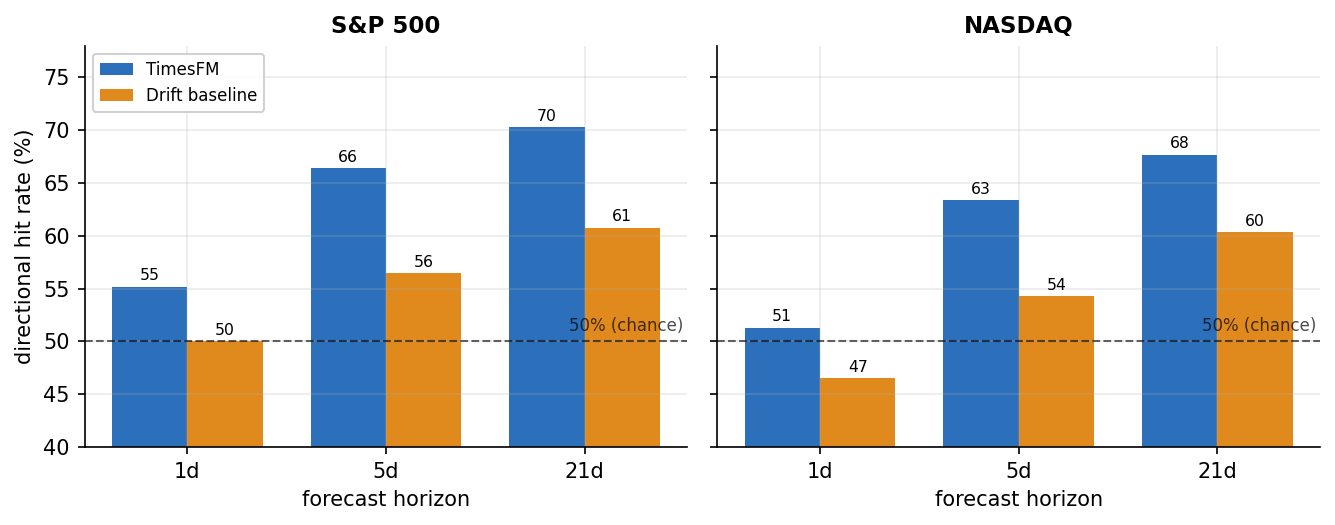
\includegraphics[width=\textwidth]{timesfm_hitrate.png}
\caption{방향 적중률: TimesFM 대 drift 기준선. TimesFM이 모든 구간\textperiodcentered 두 지수 모두에서 drift를 5--10\%p 앞선다. (random walk는 수익률 0을 예측하므로 방향 적중률이 사실상 0\%이며 방향 기준선으로 의미가 없어 생략.)}
\end{figure}

\begin{figure}[H]\centering
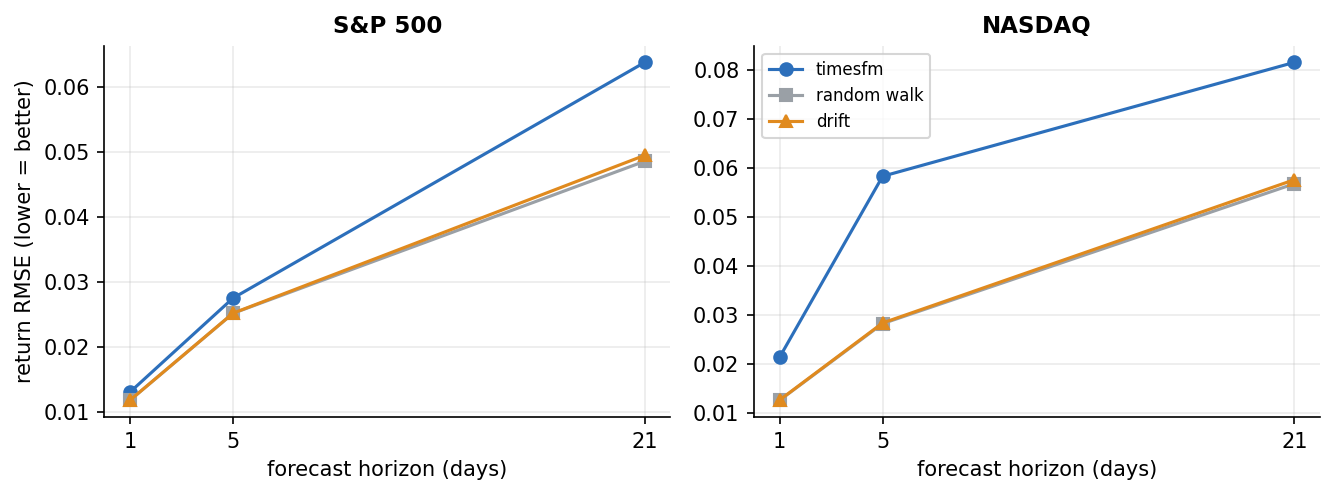
\includegraphics[width=\textwidth]{timesfm_rmse.png}
\caption{수익률 예측 RMSE. TimesFM(파랑)이 모든 구간에서 random walk\textperiodcentered drift보다 오차가 크다 --- 방향은 맞히되 변동폭을 과대추정한다.}
\end{figure}

\subsection{해석}
두 결과는 상반된 메시지를 준다. \textbf{방향성}에서 TimesFM은 단순 추세를 따라가는 drift 기준선을 일관되게(5--10\%p) 앞선다. 21일 구간의 70\% 적중률 중 상당 부분은 지수의 우상향 편향에서 오지만, drift(60.8\%) \emph{대비} 초과분은 추세를 넘어서는 방향 정보가 존재함을 시사한다(표본 $n=232$, 구간이 거의 겹치지 않아 유효표본에 가깝다). 그러나 \textbf{점 예측의 정확도}에서는 random walk보다도 RMSE가 크다(skill 전 구간 음수). 즉 \emph{언제 오르고 내릴지의 부호}는 어느 정도 잡지만 \emph{얼마나 움직일지의 크기}를 과대추정한다.

\paragraph{결론.} TimesFM은 \emph{가격/변동폭 예측기}로는 부적합하다(naive 미달). 다만 \emph{방향 신호}로서는 drift를 넘는 정보를 담고 있어, 별도 검증을 거친다면 보조 입력으로서의 가능성은 남는다. 현 단계에서 단독 참고지표로 채택하기에는 근거가 부족하다.

\section{실험 2 --- 푸리에 주기성 분석}

\subsection{방법}
로그 수익률/추세제거 잔차에 주기도(periodogram)를 계산하고, 검출된 피크가 \emph{진짜인지} AR(1) red-noise 대리표본(surrogate) 200개로 구성한 95\% 귀무 분포와 비교한다. 원본 로그 가격에 바로 FFT를 걸면 추세 에너지가 저주파를 지배하므로, 전처리 유무를 함께 본다.

\subsection{결과}
\begin{table}[H]\centering\small
\caption{전처리별 ``유의'' 피크 수(95\% AR(1) 귀무 대비)와 우연 기대치. 우연 기대치는 전체 주파수 빈의 5\%이다.}
\begin{tabular}{lrrr}
\toprule
변환 & S\&P 500 관측 & NASDAQ 관측 & 우연 기대($\approx$) \\
\midrule
\texttt{identity}        & 0   & 0   & --- \\
\texttt{demean\_logret}  & 372 & 367 & 349 / 348 \\
\texttt{detrend\_linear} & 202 & 195 & 349 / 348 \\
\bottomrule
\end{tabular}
\end{table}

\begin{figure}[H]\centering
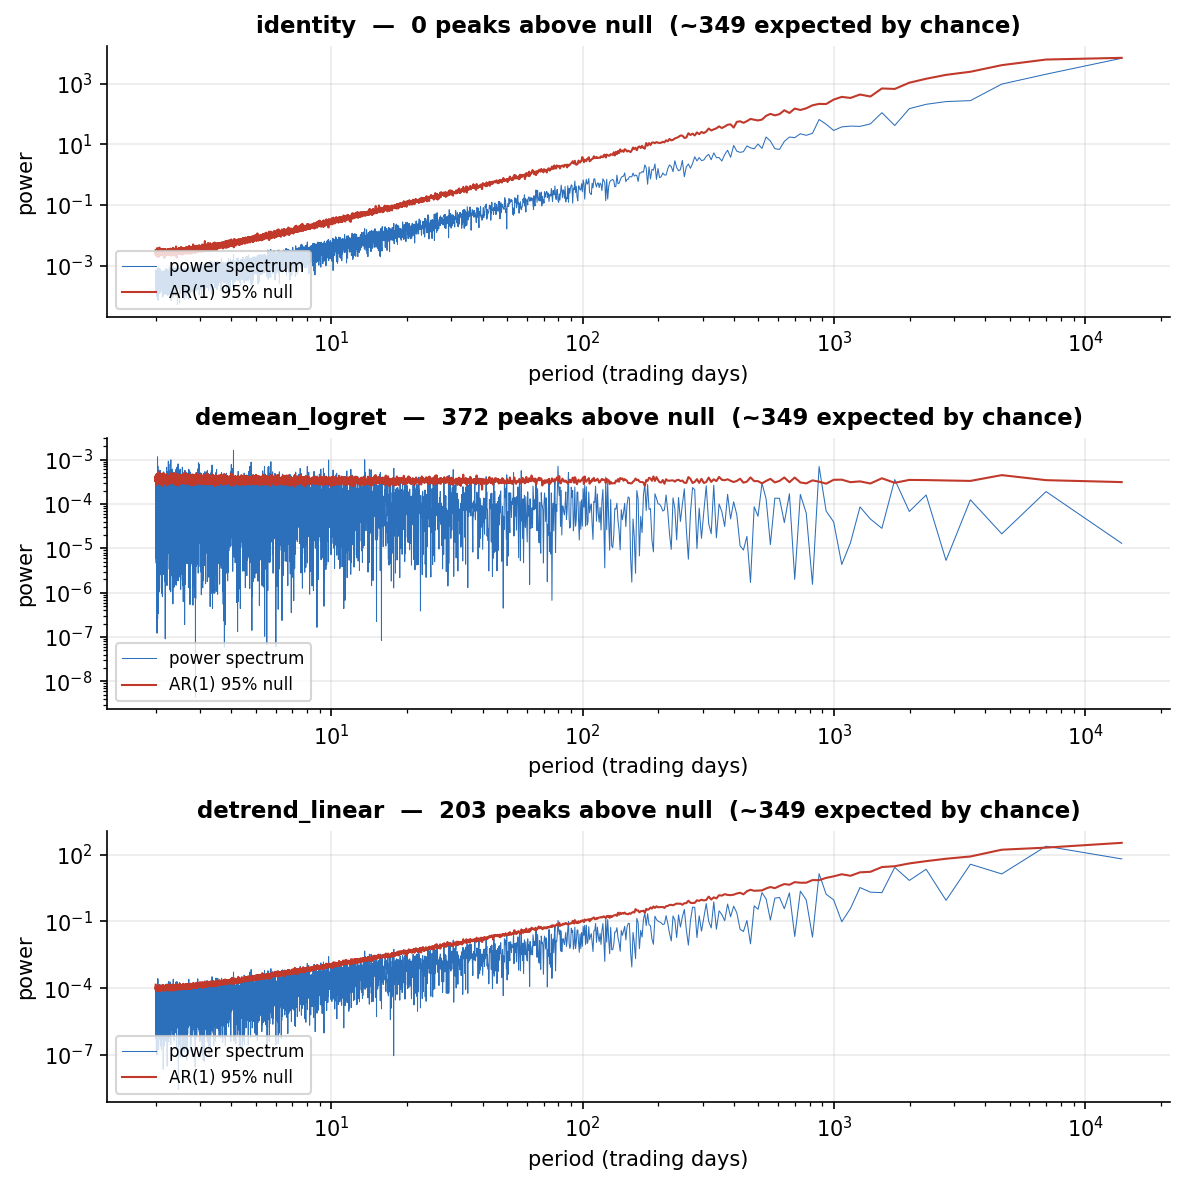
\includegraphics[width=0.92\textwidth]{fourier_spectrum_sp500.png}
\caption{S\&P~500 파워 스펙트럼(로그-로그)과 AR(1) 95\% 귀무 밴드(빨강). 무처리(\texttt{identity})는 추세가 스펙트럼을 지배해 귀무 밴드를 넘지 못한다. 전처리 후에는 다수의 피크가 밴드를 넘지만, 그 수는 우연 기대치 수준이다.}
\end{figure}

\begin{figure}[H]\centering
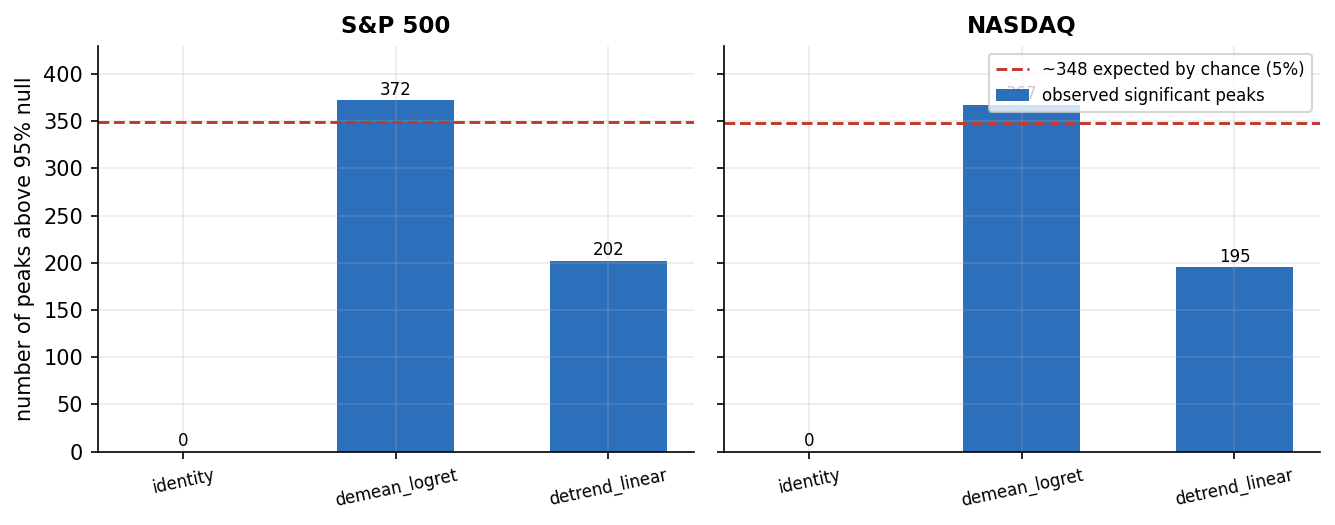
\includegraphics[width=\textwidth]{fourier_peakcount.png}
\caption{관측 피크 수(막대) 대 우연 기대치(빨간 점선). 빈당 95\% 임계값은 다중검정을 보정하지 않으므로 약 6{,}500개 빈에서 5\%($\approx$349개)가 우연히 ``유의''하게 나온다. 관측치는 이 수준 근방이거나 그 이하다.}
\end{figure}

\subsection{해석}
무처리 스펙트럼은 0개의 피크 --- 비정상(non-stationary) 추세가 모든 파워를 저주파에 모아 사실상 어떤 주기도 드러나지 않는다(전처리가 왜 필요한지 보여주는 결과). 전처리 후에는 195--372개의 피크가 ``유의''하게 나오지만, 빈당 95\% 임계값은 \emph{다중검정을 보정하지 않으므로} 약 6{,}500개 빈 중 5\%($\approx$349개)는 순전히 우연으로 유의하게 나온다. 관측된 피크 수는 이 기대치와 사실상 같은 수준이고, 어느 변환\textperiodcentered 어느 지수에서도 \emph{일관되게} 살아남는 피크는 없다.

\paragraph{결론.} 시장 지수에 신뢰할 만한 반복 주기는 발견되지 않았다. 스펙트럼은 red noise와 구분되지 않으며, 이는 사전 예상과 일치한다 --- 그리고 그 점을 깔끔하게 보여준 것 자체가 본 실험의 산출물이다.

\section{실험 3 --- 거시 이벤트 충격반응}

\subsection{방법}
``$t=0$에 발생한 충격이 이후 $h=0,1,\dots,60$ 거래일에 지수에 주는 효과''를 \emph{충격반응함수(IRF)}라는 하나의 곡선으로 보고, 거기서 \textbf{magnitude}(최대 절댓값)와 \textbf{period}(0 신뢰구간으로 복귀하는 시점, 그리고 지수감쇠 반감기)를 읽는다. 두 추정기를 함께 쓴다:
\begin{itemize}
  \item \textbf{사건 연구 CAAR} --- 사건 전 추정창의 평균 수익률을 정상값으로 보고 비정상수익률을 누적, 동일 카테고리 평균. 단순하지만 사건이 겹치거나 통제가 필요하면 약하다.
  \item \textbf{\Jorda{} 국소투영(2005)} --- 구간 $h$마다 $r(t\!\to\!t\!+\!h)=\alpha_h+\beta_h\,\text{Event}_t+\varepsilon$를 회귀, $\{\beta_h\}$가 곧 IRF. 겹치는 사건을 Newey--West(HAC) 표준오차로 통제하는 더 엄밀한 도구.
\end{itemize}

\begin{table}[H]\centering\small
\caption{큐레이션한 이벤트 목록. 2026-03 이란 사건은 분쟁이자 원유 쇼크이므로 war\textperiodcentered oil 양쪽에 등록.}
\begin{tabular}{lll}
\toprule
카테고리 & 사건(일자) \\
\midrule
war (전쟁) & 9\textperiodcentered 11(2001-09-11), 걸프전(1991-01-17), 러시아-우크라이나(2022-02-24), 이란(2026-03-01) \\
pandemic (팬데믹) & COVID 폭락(2020-02-24) \\
tariff (관세) & 미중 1차(2018-07-06), 격화(2019-05-10), 2025 관세(2025-04-02) \\
oil (원유) & 걸프 유가급등(1990-08-02), 2008 유가정점(2008-06-01), 2022 급등(2022-03-01), 이란(2026-03-01) \\
\bottomrule
\end{tabular}
\end{table}

\subsection{결과}
\begin{table}[H]\centering\small
\caption{카테고리별 충격 요약. magnitude는 CAAR의 최저점(trough), recovery는 0 신뢰구간 복귀까지의 거래일, half-life는 지수감쇠 반감기. ``---''는 60일 내 미복귀 또는 비감쇠로 정의 불가.}
\begin{tabular}{llrrrr}
\toprule
지수 & 카테고리 & $n$ & magnitude(trough) & recovery(일) & half-life(일) \\
\midrule
S\&P 500 & pandemic & 1 & $-39.8\%$ & --- & 15.5 \\
S\&P 500 & oil      & 4 & $-5.27\%$ & 39 & 11.0 \\
S\&P 500 & tariff   & 3 & $-2.92\%$ & 3  & --- \\
S\&P 500 & war      & 4 & $-0.59\%$ & 4  & --- \\
\midrule
NASDAQ  & pandemic & 1 & $-35.4\%$ & --- & 17.0 \\
NASDAQ  & oil      & 4 & $-4.70\%$ & 16 & 9.9 \\
NASDAQ  & tariff   & 3 & $-3.30\%$ & 2  & --- \\
NASDAQ  & war      & 4 & $-0.63\%$ & 4  & --- \\
\bottomrule
\end{tabular}
\end{table}

\begin{figure}[H]\centering
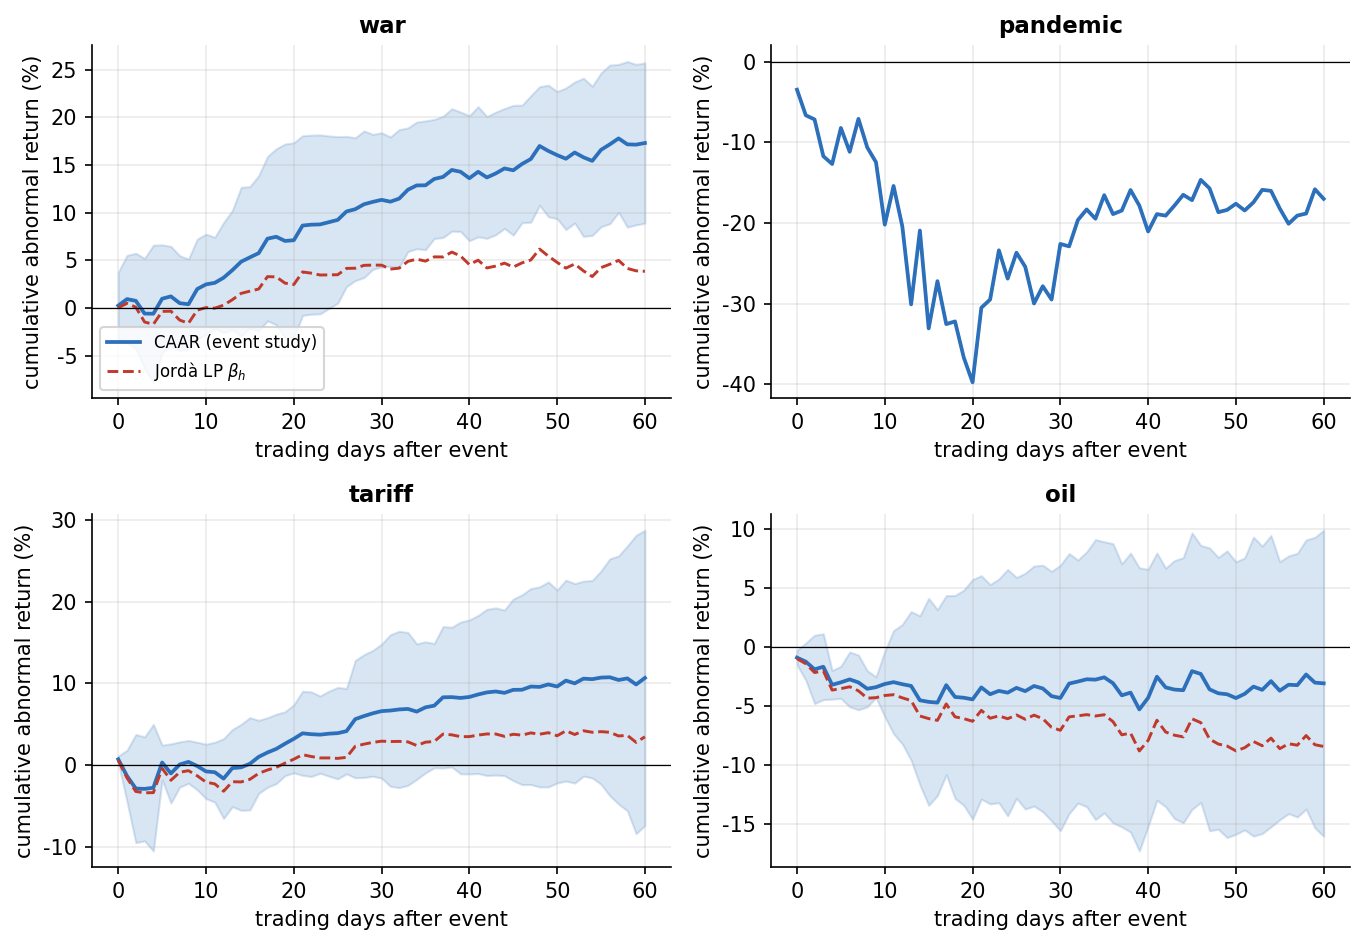
\includegraphics[width=\textwidth]{event_irf_sp500.png}
\caption{S\&P~500 카테고리별 충격반응. 파란 실선은 CAAR(사건 연구), 음영은 95\% 신뢰구간, 빨간 점선은 \Jorda{} LP $\beta_h$. 팬데믹은 단일 사건(밴드 없음).}
\end{figure}

\begin{figure}[H]\centering
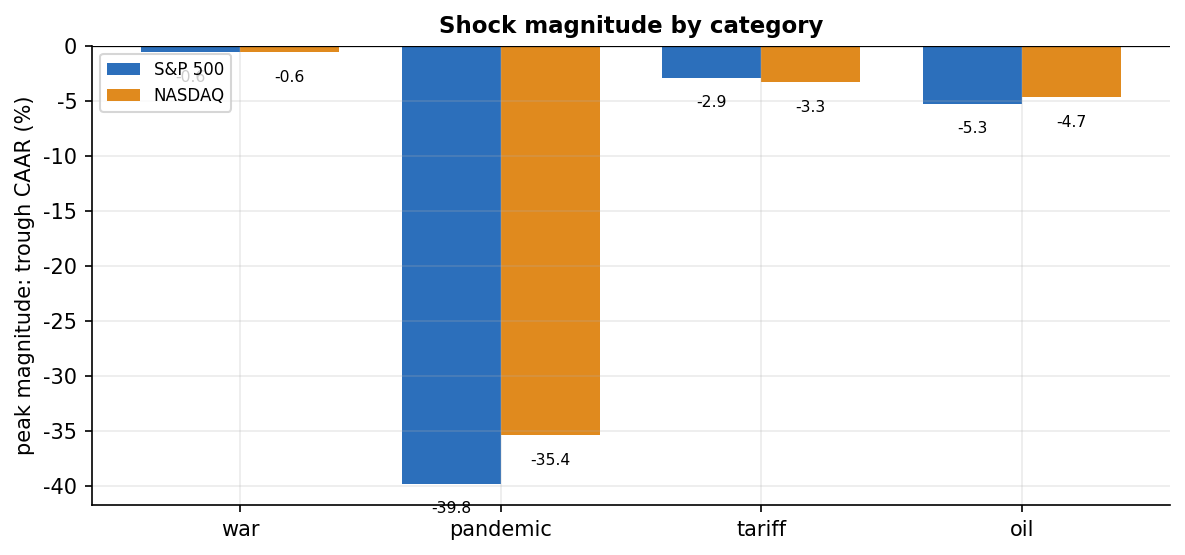
\includegraphics[width=0.8\textwidth]{event_magnitude.png}
\caption{카테고리별 충격 크기(최저점 CAAR). 팬데믹이 압도적이며, 전쟁은 매우 얕다.}
\end{figure}

\subsection{해석}
충격 유형 간 차이가 뚜렷하다.
\begin{itemize}
  \item \textbf{팬데믹}이 압도적으로 크다($-35\sim-40\%$). 단일 사건(COVID)이라 일반화는 어렵지만, 약 20거래일에 최저점을 찍고 60일 내 완전 회복하지 못한다(반감기 $\approx$15--17일).
  \item \textbf{원유}는 중간 크기($-5\%$ 안팎)의 \emph{지속적} 약세다. LP는 60일에 걸쳐 $-8\%$까지 더 음(-)으로 표류하여, 단순 CAAR보다 충격을 더 끈질기게 본다.
  \item \textbf{전쟁\textperiodcentered 관세}는 \emph{얕은 초기 하락}($-1\sim-3\%$) 뒤 표본 내에서 오히려 \emph{양(+)으로 표류}한다(그림의 war\textperiodcentered tariff 패널). 즉 이 표본에서 지정학\textperiodcentered 통상 충격은 지수의 \emph{지속적} 하락을 일으키지 않았다 --- 흔히 회자되는 ``buy the invasion'' 패턴과 일관된다.
\end{itemize}

\paragraph{주의(소표본).} war\textperiodcentered tariff\textperiodcentered oil은 사건 수가 3--4개에 불과해 신뢰구간이 매우 넓다(그림 음영). 따라서 평균(CAAR)의 부호\textperiodcentered 크기는 강하게 해석하지 말아야 하며, ``측정 \emph{방법론}이 작동함''과 ``팬데믹\textperiodcentered 원유의 음(-) 충격은 비교적 뚜렷함''까지가 안전한 결론이다.

\section{종합 논의 및 한계}

\begin{table}[H]\centering\small
\caption{세 실험 한 줄 요약.}
\begin{tabular}{lll}
\toprule
실험 & 질문 & 답 \\
\midrule
TimesFM & 참고 시그널로 쓸 만한가? & 방향 $\triangle$(drift 상회), 크기 $\times$(naive 미달) \\
푸리에 & 반복 주기가 있는가? & $\times$ (red noise 수준) \\
이벤트 임팩트 & magnitude+period 측정 가능? & $\bigcirc$ (CAAR/IRF로 정량화) \\
\bottomrule
\end{tabular}
\end{table}

\textbf{한계.} (1) 모두 \emph{지수 레벨} 분석이며 개별 종목 이벤트는 다루지 않았다. (2) TimesFM은 CPU 추론\textperiodcentered 표본 절감을 위해 21일 간격\textperiodcentered 2005년 이후로 제한했다. (3) 이벤트 표본이 작아(특히 war/tariff/oil) 통계적 검정력이 낮다. (4) 거래비용\textperiodcentered 슬리피지를 반영한 매매 시뮬레이션은 범위 밖이다.

\textbf{후속 제안.} TimesFM을 \emph{순수 방향 분류기}로 always-long 기준선과 정식 비교(맥니마 검정 등); 이벤트 카테고리별 표본 확충 후 LP 신뢰구간 재추정; 충격의 \emph{비대칭}(상승 vs 하락 쇼크) 분리.

\section{결론}
세 실험은 각각 정직한 답을 냈다. \emph{TimesFM}은 가격 예측기로는 naive를 못 이기지만 방향성에는 추세 이상의 정보가 있고, \emph{푸리에}로는 신뢰할 주기가 없으며, \emph{이벤트 충격}은 사건 연구와 국소투영으로 크기\textperiodcentered 지속을 정량화할 수 있음을 확인했다. 셋 중 Croesus에 바로 ``참고 지표''로 넣을 만한 것은 없으나, 이벤트 충격반응 프레임워크는 추가 데이터와 함께 발전시킬 가치가 있다.

\vfill
\footnotesize\noindent\textbf{재현.} 결과 산출물(CSV/PNG)은 git에서 제외되어 있다. 저장소 루트에서 다음으로 재생성한다: \texttt{python -m experiments.market\_signals.\{fourier,event\_impact,timesfm\_eval\}.run} (TimesFM은 전용 venv 필요\textperiodcentered 느림). 본 보고서의 그림은 \texttt{python -m experiments.market\_signals.report.make\_figures}로 생성한다. 그림 축 라벨은 폰트 호환을 위해 영문으로 유지하고 한국어 설명은 캡션에 둔다. 단위 테스트 16개 통과. 설계\textperiodcentered 계획 문서는 \texttt{docs/superpowers/}에 있다.

\end{document}
